\graphicspath{{images/}}

\section*{Komplexitätstheorie}

\begin{definition}{Quantitative Gesetze und Grenzen}

    \begin{itemize}
    \item Zeitkomplexität: Laufzeit des besten Programms
    \item Platzkomplexität: Speicherplatz des besten Programms
    \item Beschreibungskomplexität: Länge des kürzesten Programms
    \end{itemize}
\end{definition}

\begin{theorem}{Zeitbedarf}
    von $M$ auf Eingaben der Länge $n \in \mathbb{N}$ 
    
    im schlechtesten Fall: $\operatorname{Time}_{M}(n)=\max \left\{\operatorname{Time}_{M}(\omega)|| \omega \mid=n\right\}$
    
    \vspace{1mm}

    Sei $M$ eine TM, die immer hält und sei die Eingabe $\omega \in \Sigma^{*}$
    
    Zeitbedarf von $M$ auf $\omega$: Time $_{M}(\omega)=$ Anzahl Konfigurationsübergänge in der Berechnung von $M$ auf $\omega$
\end{theorem}

\begin{KR}{P vs NP}
    Klassifizierung von Problemen\\
    Ein Problem $U$ heisst in Polynomzeit lösbar, wenn es eine obere Schranke $O\left(n^{c}\right)$ gibt für eine Konstante $c \geq 1$.
    \begin{itemize}
    \item $P \doteq $ Lösung finden in Polynomzeit
    \item $N P \doteq $ Lösung verifizieren in Polynomzeit
    \end{itemize}
\end{KR}

\begin{remark}
    \textcolor{pink}{ACHTUNG:} NP heisst nicht «nicht-polynomial» sondern «nicht-deterministisch polynomial»
\end{remark}

\begin{concept}{NP-schwer und NP-vollständig}\\
    \begin{minipage}{0.6\linewidth}
        Eine Sprache $L$ heisst $N P$-schwer, falls für alle Sprachen $L^{\prime} \in N P$ gilt, \\dass $L^{\prime} \preccurlyeq_{p} L$
        
        Eine Sprache $L$ heisst NP-vollständig, falls $L \in N P$ und $L$ ist NP-schwer.
    \end{minipage}
    \begin{minipage}{0.38\linewidth}
        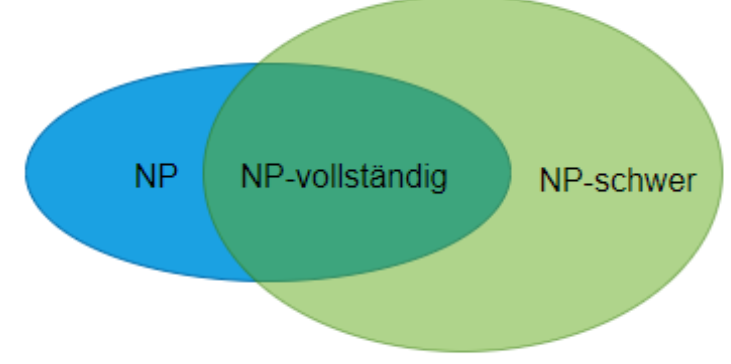
\includegraphics[width=1\linewidth]{images/p_vs_np.png}
    \end{minipage}
\end{concept}

\begin{remark}
    $P \subset N P $ gilt, aber $P \neq \N P$ noch nicht bewiesen
\end{remark}

\begin{definition}{Polynomzeit-Verifizierer}
    Überprüft die Eingaben in einem Problem\\
    Zeuge: Informationen einer gültigen Eingabe
\end{definition}

\begin{KR}{Asymptotische Komplexitätsmessung}
    $O$-Notation
    \begin{itemize}
        \item $f \in O(g)$: $f(n) \leq c \cdot g(n)$
        \begin{itemize}
            \item f wächst asymptotisch nicht schneller als $g$
        \end{itemize}
        \item $f \in \Omega(g)$: $f(n) \geq \frac{1}{d} \cdot g(n)$
        \begin{itemize}
            \item f wächst asymptotisch mindestens so schnell wie $g$
        \end{itemize}
        \item $f \in \Theta(g)$: Es gilt $f(n) \in O(g(n))$ und $f(n) \in \Omega(g(n))$
        \begin{itemize}
            \item $f$ und $g$ sind asymptotisch gleich
        \end{itemize}
    \end{itemize}
\end{KR}

\begin{concept}{Schranken für die Zeitkomplexität von U}
    \begin{itemize}
    \item $O(f(n))$ ist eine obere Schranke, falls Eine TM existiert, die $U$ löst und eine Zeitkomplexität in $O(f(n))$ hat.
    \item $\Omega(g(n))$ ist eine untere Schranke, falls Für alle TM $M$, die $U$ lösen, gilt dass $\operatorname{Time}_{\mathrm{M}}(n) \in \Omega(g(n))$
    \end{itemize}
\end{concept}

\begin{formula}{Rechenregeln}
    \begin{itemize}
    \item Konstante Vorfaktoren $c$ ignorieren $(c \in O(1))$
    \item Bei Polynomen ist nur die höchste Potenz entscheidend
    \item Transitiv:
            $f(n) \in O(g(n)) \wedge g(n) \in O(h(n)) \rightarrow f(n) \in O(h(n))$
    \end{itemize}
\end{formula}

\begin{KR}{Übersicht wichtigste Laufzeiten}

    $O(1) < O(\log (\log n)) < O(\sqrt{\log n}) < O(\log \sqrt{n}) < O(\log n)$\\ 
    $< O(\sqrt{n}) < O(n) < O(n \log n) < O(n^{2}) < O(n^{3})$ \\
    $< O(n^c) < O(2^{n}) < O(n!) < O(n^n)$
\end{KR}

\vspace{2mm}

{\footnotesize
\textcolor{pink}{good luck <3}}


